
\documentclass[letterpaper, reqno,12pt]{article}
\usepackage[margin=1.0in]{geometry}
\usepackage[dvipsnames]{xcolor}
\usepackage{latexsym,amsmath,amssymb}
\usepackage{fancyhdr}
\usepackage{amsthm}
\usepackage[linesnumbered,lined,boxed,commentsnumbered]{algorithm2e}
\usepackage{dsfont}
\usepackage{graphicx}
\usepackage{hyperref}
\usepackage{lmodern}
\usepackage[numbers]{natbib}
\usepackage{listings}% http://ctan.org/pkg/listings
\lstset{
  basicstyle=\ttfamily,
  columns=fullflexible,
  mathescape
}
\usepackage{enumitem}
\usepackage{subcaption}
\usepackage{tikz}
\usetikzlibrary{decorations.pathreplacing,calligraphy}
\usetikzlibrary{patterns}

\allowdisplaybreaks

\newcommand{\RR}{\mathbb{R}}
\newcommand{\CC}{\mathbb{C}}
\newcommand{\ZZ}{\mathbb{Z}}
\newcommand{\QQ}{\mathbb{Q}}
\newcommand{\NN}{\mathbb{N}}
\newcommand{\mynote}[3][red]
  {{\color{#1} \fbox{\bfseries\sffamily\scriptsize#2}
  {\small$\blacktriangleright$\textsf{\emph{#3}}$\blacktriangleleft$}}~}
\newcommand{\yp}[1]{\mynote{YP}{#1}}
\DeclareMathOperator{\conv}{conv}
\DeclareMathOperator{\charcone}{char.cone}
\DeclareMathOperator{\STAB}{STAB}
\DeclareMathOperator{\Down}{Down}
\DeclareMathOperator{\lca}{lca}
\DeclareMathOperator{\LPO}{LPO}
\DeclareMathOperator{\OPT}{OPT}
\DeclareMathOperator{\LHS}{LHS}
\DeclareMathOperator{\RHS}{RHS}
\DeclareMathOperator{\tr}{tr}
\DeclareMathOperator{\vol}{vol}
\DeclareMathOperator{\argmin}{arg\,min}
\DeclareMathOperator{\argmax}{arg\,max}
\DeclareMathOperator{\poly}{poly}
\DeclareMathOperator{\Span}{span}
\DeclareMathOperator{\supp}{supp}
\DeclareMathOperator{\dist}{dist}
\begin{document}
\pagenumbering{arabic}
\title{KKM-Type Theorems and Their Applications\footnote{Lecturer: Shira Zerbib, Iowa State University, \href{mailto:zerbib@iastate.edu}{zerbib@iastate.edu}.}}
\author{Yuchong Pan\thanks{MIT, \href{mailto:yuchong@mit.edu}{yuchong@mit.edu}.}}
\date{\today}
\newtheorem{theorem}{Theorem}
\newtheorem{lemma}[theorem]{Lemma}
\newtheorem{corollary}[theorem]{Corollary}
\newtheorem{problem}[theorem]{Problem}
\theoremstyle{definition} \newtheorem{definition}[theorem]{Definition}
\maketitle
%

\section{Two Problems}

First, we consider two seemingly unrelated problems.

\subsection{A Colorful Gallai's Theorem}

\begin{definition}
  Let $\mathcal F$ be a finite family of compact intervals in $\RR$. Define the \emph{matching number} of $\mathcal F$, denoted by $\nu(\mathcal F)$, to be the maximum number of pairwise disjoint intervals in $\mathcal F$. Define the \emph{covering number} of $\mathcal F$, denoted by $\tau(\mathcal F)$, to be the minimum number of points needed to intersect all intervals in $\mathcal F$. A \emph{matching} is a set of pairwise disjoint intervals.
\end{definition}

Figure \ref{fig:nu-tau} gives two examples.

\begin{figure}[h]
  \centering
  \begin{subfigure}[b]{0.45\textwidth}
    \centering
    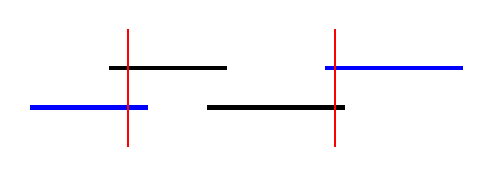
\begin{tikzpicture}
      \draw[blue, ultra thick] (0, 0) -- (1.5, 0);
      \draw[ultra thick] (1, .5) -- (2.5, .5);
      \draw[ultra thick] (2.25, 0) -- (4, 0);
      \draw[blue, ultra thick] (3.75, .5) -- (5.5, .5);
      \draw[red, thick] (1.25, -.5) -- (1.25, 1);
      \draw[red, thick] (3.875, -.5) -- (3.875, 1);
    \end{tikzpicture}
    \caption{$\nu(\mathcal F) = \tau(\mathcal F) = 2$.}
  \end{subfigure}
  \hfill
  \begin{subfigure}[b]{0.45\textwidth}
    \centering
    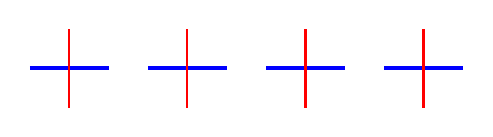
\begin{tikzpicture}
      \draw[blue, ultra thick] (0, 0) -- (1, 0);
      \draw[blue, ultra thick] (1.5, 0) -- (2.5, 0);
      \draw[blue, ultra thick] (3, 0) -- (4, 0);
      \draw[blue, ultra thick] (4.5, 0) -- (5.5, 0);
      \draw[red, thick] (.5, -.5) -- (.5, .5);
      \draw[red, thick] (2, -.5) -- (2, .5);
      \draw[red, thick] (3.5, -.5) -- (3.5, .5);
      \draw[red, thick] (5, -.5) -- (5, .5);
    \end{tikzpicture}
    \caption{$\nu(\mathcal F) = \tau(\mathcal F) = 4$.}
  \end{subfigure}
  \caption{Two examples of the matching number and the covering number of a finite family of compact intervals in $\RR$, where red vertical lines denote a minimum set of points that intersect all intervals in $\mathcal F$, and blue intervals denote a maximum set of pairwise disjoint intervals.}
  \label{fig:nu-tau}
\end{figure}

\begin{theorem}[Gallai, 1960]
  If $\mathcal F$ is a finite family of compact intervals in $\RR$, then $\tau(\mathcal F) = \nu(\mathcal F)$.
\end{theorem}

It is trivial to see that $\tau(\mathcal F) \geq \nu(\mathcal F)$, as any set of $k$ pairwise disjoint intervals requires $k$ points to intersect all the intervals in the set. We reformulate Gallai's theorem as follows:

\begin{theorem}[Gallai, 1960]
  Let $\mathcal F$ be a finite family of compact intervals in $\RR$. If $\tau(\mathcal F) > k$, then there exists a matching in $\mathcal F$ of size $k + 1$.
\end{theorem}

We consider the following colorful version of Gallai's theorem:

\begin{problem}
  Let $\mathcal F_1, \ldots, \mathcal F_{k + 1}$ be $k + 1$ families of intervals in $\RR$ such that $\tau(\mathcal F_i) > k$ for all $i \in [k + 1]$. Can one find a \emph{rainbow matching}, where a \emph{rainbow matching} is a matching $\mathcal M$ such that $|\mathcal M \cap \mathcal F_i| = 1$ for all $i \in [k + 1]$?
\end{problem}

Figure \ref{fig:colorful-gallai} gives an example of the colorful version of Gallai's theorem.

\begin{figure}[h]
  \centering
  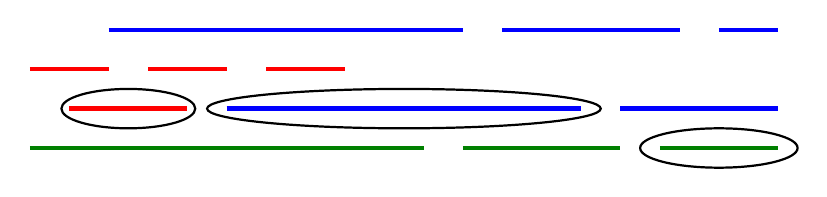
\begin{tikzpicture}
    \draw[Green, ultra thick] (0, 0) -- (5, 0);
    \draw[Green, ultra thick] (5.5, 0) -- (7.5, 0);
    \draw[Green, ultra thick] (8, 0) -- (9.5, 0);
    \draw[red, ultra thick] (0, 1) -- (1, 1);
    \draw[red, ultra thick] (1.5, 1) -- (2.5, 1);
    \draw[red, ultra thick] (3, 1) -- (4, 1);
    \draw[red, ultra thick] (.5, .5) -- (2, .5);
    \draw[blue, ultra thick] (2.5, .5) -- (7, .5);
    \draw[blue, ultra thick] (7.5, .5) -- (9.5, .5);
    \draw[blue, ultra thick] (1, 1.5) -- (5.5, 1.5);
    \draw[blue, ultra thick] (6, 1.5) -- (8.25, 1.5);
    \draw[blue, ultra thick] (8.75, 1.5) -- (9.5, 1.5);
    \draw[thick] (1.25, .5) ellipse (.85 and .25);
    \draw[thick] (4.75, .5) ellipse (2.5 and .25);
    \draw[thick] (8.75, 0) ellipse (1 and .25);
  \end{tikzpicture}
  \caption{An example of the colorful Gallai's theorem, where each family is denoted by a distinct color, the covering number of each family is greater than $2$, and a rainbow matching is circled.}
  \label{fig:colorful-gallai}
\end{figure}

\subsection{Fair Division of a Cake}

Consider a cake identified by $[0, 1]$ and $n$ players. Given any partition of the cake, each player gives a list of pieces they prefer in that partition. We say that a player is \emph{hungry} if they prefer a piece of positive length in any partition. Figure \ref{fig:empty} gives a partition of the cake with an empty piece.

\begin{figure}[h]
  \centering
  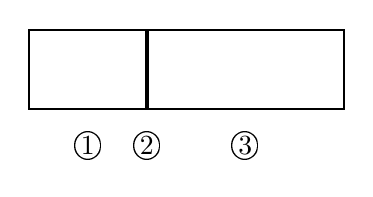
\begin{tikzpicture}
    \draw[thick] (0, 0) -- (4, 0) -- (4, 1) -- (0, 1) -- cycle;
    \draw[ultra thick] (1.5, 0) -- (1.5, 1);
    \node at (.75, -.5) {\textcircled{\raisebox{-1pt}{1}}};
    \node at (1.5, -.5) {\textcircled{\raisebox{-1pt}{2}}};
    \node at (2.75, -.5) {\textcircled{\raisebox{-1pt}{3}}};
  \end{tikzpicture}
  \caption{A partition of the cake, where the second piece is an empty piece.}
  \label{fig:empty}
\end{figure}

We say that a preference list is \emph{closed} if the following holds: if the player refers piece $i$ in a converging sequence of partitions, then they prefer piece $i$ also in the limiting partition. See Figure \ref{fig:closed} for an illustration.

\begin{figure}[h]
  \centering
  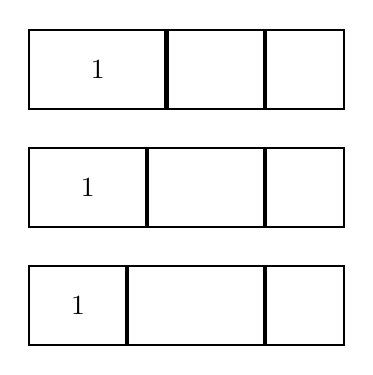
\begin{tikzpicture}
    \draw[thick] (0, 3) -- (4, 3) -- (4, 4) -- (0, 4) -- cycle;
    \draw[ultra thick] (1.75, 3) -- (1.75, 4);
    \draw[ultra thick] (3, 3) -- (3, 4);
    \draw[thick] (0, 1.5) -- (4, 1.5) -- (4, 2.5) -- (0, 2.5) -- cycle;
    \draw[ultra thick] (1.5, 1.5) -- (1.5, 2.5);
    \draw[ultra thick] (3, 1.5) -- (3, 2.5);
    \draw[thick] (0, 0) -- (4, 0) -- (4, 1) -- (0, 1) -- cycle;
    \draw[ultra thick] (1.25, 0) -- (1.25, 1);
    \draw[ultra thick] (3, 0) -- (3, 1);
    \node at (.875, 3.5) {$1$};
    \node at (.75, 2) {$1$};
    \node at (.625, .5) {$1$};
  \end{tikzpicture}
  \caption{Illustrating the concept of a closed preference list, where the three partitions indicate a converging sequence of partitions. If the first player prefers the first piece in every partition in this sequence, then they must prefer the first piece in the limiting partition.}
  \label{fig:closed}
\end{figure}

Moreover, we say that a division (i.e., a partition) is \emph{envy-free} if each player has a distinct piece in their preference list.

\begin{theorem}[Su, 1980]
  If every player is hungry, and if the preference list of each player is closed, then an envy-free division exists.
\end{theorem}

\section{Sperner's Lemma, Brouwer's Fixed Point Theorem, and the KKM Theorem}

In this section, we state Sperner's lemma, Brouwer's fixed point theorem, and the KKM theorem. These three results are equivalent and imply one another. We shall prove Sperner's lemma and that Brouwer's fixed point theorem implies that the KKM theorem. The other implications are left as exercises.

\begin{theorem}[Brouwer, 1914]
  Any continuous map $f$ from a closed ball to itself has a fixed point, namely a point $x$ with $f(x) = x$.
\end{theorem}

\subsection{Sperner's Lemma}

\begin{definition}
  \noindent
  \begin{enumerate}[itemsep=0pt]
    \item An \emph{$n$-dimensional simplex} is the convex hull of $n + 1$ affinely independent points in $\RR^{n + 1}$.
    \item The \emph{standard $n$-dimensional simplex} is defined to be $\Delta^n = \conv\{ e_1, \ldots, e_{n + 1} \} \subseteq \RR^{n + 1}$.
    \item A \emph{face} of a simplex is the convex hull of a subset of the points defining the simplex. The \emph{dimension} of a face is the number of points defining it minus $1$.
    \item A \emph{triangulation} of $\Delta^n$ is a subdivision of $\Delta^n$ into simplices.
  \end{enumerate}
\end{definition}

Figure \ref{fig:triangulation} gives an example of a triangulation of $\Delta^2$.

\begin{figure}[h]
  \centering
  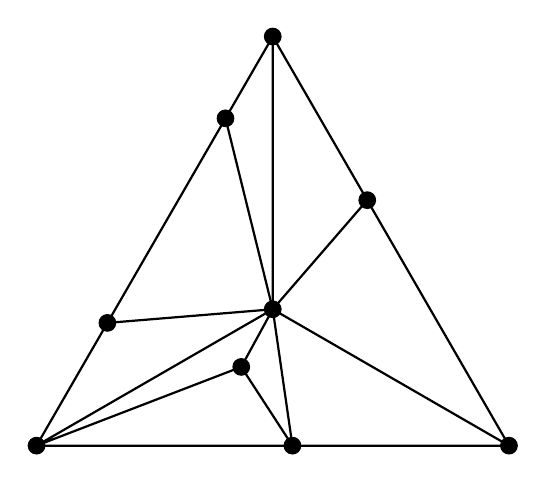
\begin{tikzpicture}
    \draw[thick] (-3, 0) -- (3, 0) -- (0, 5.196) -- cycle;
    \draw[fill=black] (-3, 0) circle (3pt);
    \draw[fill=black] (3, 0) circle (3pt);
    \draw[fill=black] (0, 5.196) circle (3pt);
    \draw[fill=black] (0, 1.732) circle (3pt);
    \draw[fill=black] (.25, 0) circle (3pt);
    \draw[fill=black] (-.4, 1) circle (3pt);
    \draw[fill=black] (1.2, 3.118) circle (3pt);
    \draw[fill=black] (-.6, 4.157) circle (3pt);
    \draw[fill=black] (-2.1, 1.559) circle (3pt);
    \draw[thick] (3, 0) -- (0, 1.732) -- (-3, 0) -- (-.4, 1) -- (.25, 0) -- (0, 1.732) -- (-.4, 1);
    \draw[thick] (0, 5.196) -- (0, 1.732) -- (1.2, 3.118);
    \draw[thick] (-.6, 4.157) -- (0, 1.732) -- (-2.1, 1.559);
  \end{tikzpicture}
  \caption{An example of a triangulation of $\Delta^2$.}
  \label{fig:triangulation}
\end{figure}

\begin{definition}
  Let $T$ be a triangulation of $\Delta^n$. A \emph{Sperner coloring} of $T$ is a map $\lambda : V(T) \to [n + 1]$ such that
  \begin{enumerate}[itemsep=0pt]
    \item every vertex of $\Delta^n$ must get a distinct color (i.e., $\lambda(e_1), \ldots, \lambda(e_{n + 1})$ are all distinct);
    \item $\lambda(v) \in \lambda(V(\supp(v)))$ for all $v \in T$, where the \emph{support} of a point $v \in \Delta^n$, denoted by $\supp(v)$, is the minimal face in $\Delta^n$ containing $v$.
  \end{enumerate}
\end{definition}

Figure \ref{fig:supp} gives an example of the support of a point in $\Delta^2$. Figure \ref{fig:sperner} gives an example of a Sperner coloring of the triangulation in Figure \ref{fig:triangulation}.

\begin{figure}[h]
  \centering
  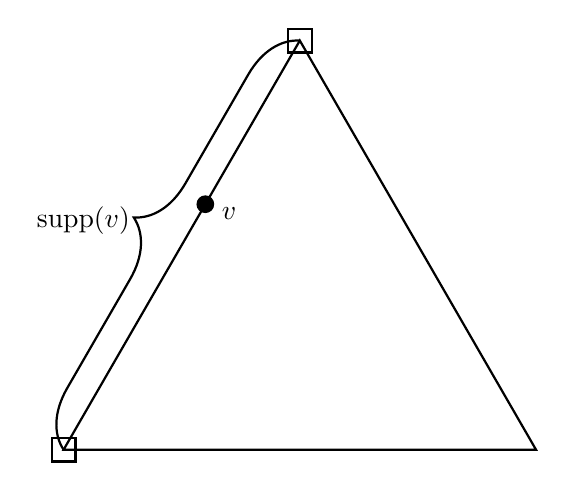
\begin{tikzpicture}
    \draw[thick] (-3, 0) -- (3, 0) -- (0, 5.196) -- cycle;
    \draw[fill=black] (-1.2, 3.118) circle (3pt);
    \node at (-.9, 3) {$v$};
    \draw[thick] (-3.15, -.15) rectangle ++(.3, .3);
    \draw[thick] (-.15, 5.046) rectangle ++(.3, .3);
    \draw[thick, decorate, decoration={brace, amplitude=20pt}] (-3, 0) -- (0, 5.196) node[midway, above left, xshift=-15pt] {$\supp(v)$};
  \end{tikzpicture}
  \caption{An example of the support of a point $v$ in $\Delta^2$, so the color of $v$ must be one of the colors of the boxed vertices (which are the vertices of $\supp(v)$).}
  \label{fig:supp}
\end{figure}

\begin{figure}[h]
  \centering
  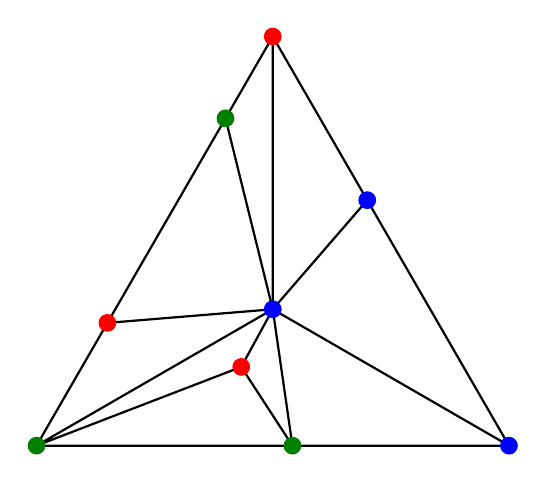
\begin{tikzpicture}
    \draw[thick] (-3, 0) -- (3, 0) -- (0, 5.196) -- cycle;
    \draw[thick] (3, 0) -- (0, 1.732) -- (-3, 0) -- (-.4, 1) -- (.25, 0) -- (0, 1.732) -- (-.4, 1);
    \draw[thick] (0, 5.196) -- (0, 1.732) -- (1.2, 3.118);
    \draw[thick] (-.6, 4.157) -- (0, 1.732) -- (-2.1, 1.559);
    \draw[Green, fill=Green] (-3, 0) circle (3pt);
    \draw[blue, fill=blue] (3, 0) circle (3pt);
    \draw[red, fill=red] (0, 5.196) circle (3pt);
    \draw[blue, fill=blue] (0, 1.732) circle (3pt);
    \draw[Green, fill=Green] (.25, 0) circle (3pt);
    \draw[red, fill=red] (-.4, 1) circle (3pt);
    \draw[blue, fill=blue] (1.2, 3.118) circle (3pt);
    \draw[Green, fill=Green] (-.6, 4.157) circle (3pt);
    \draw[red, fill=red] (-2.1, 1.559) circle (3pt);
  \end{tikzpicture}
  \caption{An example of a triangulation of $\Delta^2$.}
  \label{fig:sperner}
\end{figure}

\begin{definition}
  A \emph{rainbow simplex} in a triangulation is a simplex whose vertices are colored by all colors $1, \ldots, n + 1$.
\end{definition}

\begin{theorem}[Sperner, 1928]
  Let $T$ be a triangulation of $\Delta^n$. Let $\lambda : V(T) \to [n + 1]$ be a Sperner coloring. Then the number of rainbow simplices is odd.
\end{theorem}

\begin{proof}
  If $n = 0$, then $\Delta^0$ is a single point, so the theorem is trivially true.

  If $n = 1$, then $\Delta^1$ is the interval $[0, 1]$, and any triangulation partitions $[0, 1]$. Since $0$ and $1$ are colored by two different colors in a Sperner coloring, then the colors of the vertices from $0$ to $1$ must switch an odd number of times. See Figure \ref{fig:sperner-1} for an illustration.

  \begin{figure}[h]
    \centering
    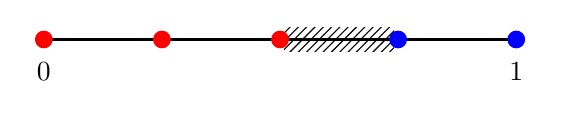
\begin{tikzpicture}
      \draw[thick] (0, 0) -- (6, 0);
      \fill[pattern=north east lines] (3.05, -0.15) rectangle ++(1.4, .3);
      \draw[red, fill=red] (0, 0) circle (3pt) node[below, yshift=-5pt] {\color{black} $0$};
      \draw[red, fill=red] (1.5, 0) circle (3pt);
      \draw[red, fill=red] (3, 0) circle (3pt);
      \draw[blue, fill=blue] (4.5, 0) circle (3pt);
      \draw[blue, fill=blue] (6, 0) circle (3pt) node[below, yshift=-5pt] {\color{black} $1$};
    \end{tikzpicture}
    \caption{Illustrating the proof of Sperner's lemma for the case $n = 1$, where changes of the colors are shaded.}
    \label{fig:sperner-1}
  \end{figure}

  We proceed by induction on $n$. For $n \geq 2$, consider the face of $\Delta^n$ colored by $1, 2, \ldots, n$. By induction, it has odd many rainbow $(n - 1)$-simplices, colored by $1, 2, \ldots, n$. Define an auxiliary graph $G$, where the vertices are the simplices of $T$ plus one other vertex $v^*$ in the outer face, and two vertices in $G$ are connceted by an edge if they share an $(n - 1)$-face (see Figure \ref{fig:graph} for an illustration for the case $n = 2$). Since $\sum_{v \in V(G)} \deg(v) = 2|E(G)|$ is even and since $\deg(v^*)$ is odd, then $G$ has odd many other vertices of odd degree, corresponding to rainbow simplices (see Figure \ref{fig:corr} for the correspondence between the coloring of a simplex and the degree of its vertex in the auxiliary graph in the case $n = 2$). This completes the induction step.

  \begin{figure}[h]
    \centering
    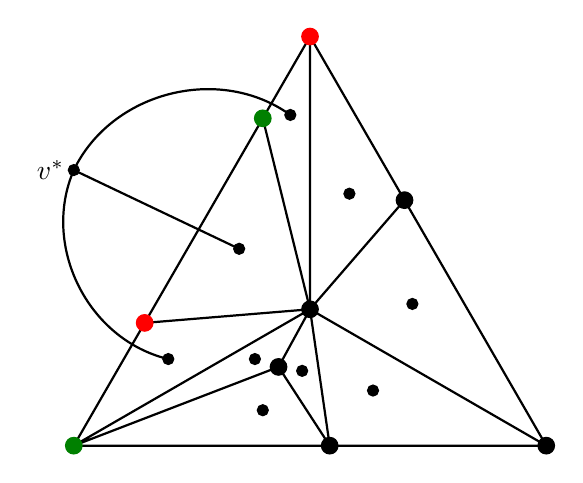
\begin{tikzpicture}
      \draw[thick] (-3, 0) -- (3, 0) -- (0, 5.196) -- cycle;
      \draw[thick] (3, 0) -- (0, 1.732) -- (-3, 0) -- (-.4, 1) -- (.25, 0) -- (0, 1.732) -- (-.4, 1);
      \draw[thick] (0, 5.196) -- (0, 1.732) -- (1.2, 3.118);
      \draw[thick] (-.6, 4.157) -- (0, 1.732) -- (-2.1, 1.559);
      \draw[Green, fill=Green] (-3, 0) circle (3pt);
      \draw[fill=black] (3, 0) circle (3pt);
      \draw[red, fill=red] (0, 5.196) circle (3pt);
      \draw[fill=black] (0, 1.732) circle (3pt);
      \draw[fill=black] (.25, 0) circle (3pt);
      \draw[fill=black] (-.4, 1) circle (3pt);
      \draw[fill=black] (1.2, 3.118) circle (3pt);
      \draw[Green, fill=Green] (-.6, 4.157) circle (3pt);
      \draw[red, fill=red] (-2.1, 1.559) circle (3pt);
      \draw[fill=black] (-.6, .45) circle (2pt);
      \draw[fill=black] (-.1, .95) circle (2pt);
      \draw[fill=black] (-.7, 1.1) circle (2pt);
      \draw[fill=black] (-1.8, 1.1) circle (2pt);
      \draw[fill=black] (-.9, 2.5) circle (2pt);
      \draw[fill=black] (-.25, 4.2) circle (2pt);
      \draw[fill=black] (.5, 3.2) circle (2pt);
      \draw[fill=black] (.8, .7) circle (2pt);
      \draw[fill=black] (1.3, 1.8) circle (2pt);
      \draw[fill=black] (-3, 3.5) circle (2pt) node[left] {$v^*$};
      \draw[thick] (-3, 3.5) to[bend left=50] (-.25, 4.2);
      \draw[thick] (-3, 3.5) -- (-.9, 2.5);
      \draw[thick] (-3, 3.5) to[bend right=50] (-1.8, 1.1);
    \end{tikzpicture}
    \caption{Illustrating the auxiliary graph in the proof of Sperner's lemma for the case $n = 2$.}
    \label{fig:graph}
  \end{figure}

  \begin{figure}[h]
    \centering
    \begin{subfigure}[b]{.24\textwidth}
      \centering
      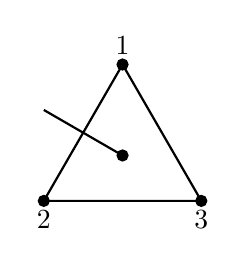
\begin{tikzpicture}
        \draw[fill=black] (-1, 0) circle (2pt) node[below] {$2$};
        \draw[fill=black] (1, 0) circle (2pt) node[below] {$3$};
        \draw[fill=black] (0, 1.732) circle (2pt) node[above] {$1$};
        \draw[thick] (-1, 0) -- (1, 0) -- (0, 1.732) -- cycle;
        \draw[fill=black] (0, .577) circle (2pt);
        \draw[thick] (0, .577) -- (-1, 1.155);
      \end{tikzpicture}
    \end{subfigure}
    \hfill
    \begin{subfigure}[b]{.24\textwidth}
      \centering
      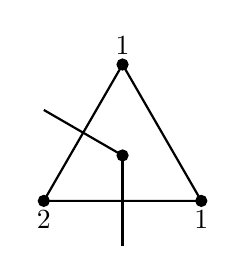
\begin{tikzpicture}
        \draw[fill=black] (-1, 0) circle (2pt) node[below] {$2$};
        \draw[fill=black] (1, 0) circle (2pt) node[below] {$1$};
        \draw[fill=black] (0, 1.732) circle (2pt) node[above] {$1$};
        \draw[thick] (-1, 0) -- (1, 0) -- (0, 1.732) -- cycle;
        \draw[fill=black] (0, .577) circle (2pt);
        \draw[thick] (0, .577) -- (-1, 1.155);
        \draw[thick] (0, .577) -- (0, -.577);
      \end{tikzpicture}
    \end{subfigure}
    \hfill
    \begin{subfigure}[b]{.24\textwidth}
      \centering
      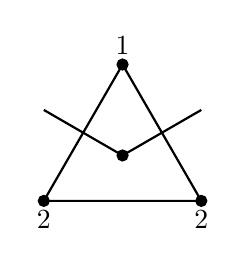
\begin{tikzpicture}
        \draw[fill=black] (-1, 0) circle (2pt) node[below] {$2$};
        \draw[fill=black] (1, 0) circle (2pt) node[below] {$2$};
        \draw[fill=black] (0, 1.732) circle (2pt) node[above] {$1$};
        \draw[thick] (-1, 0) -- (1, 0) -- (0, 1.732) -- cycle;
        \draw[fill=black] (0, .577) circle (2pt);
        \draw[thick] (0, .577) -- (-1, 1.155);
        \draw[thick] (0, .577) -- (1, 1.155);
      \end{tikzpicture}
    \end{subfigure}
    \hfill
    \begin{subfigure}[b]{.24\textwidth}
      \centering
      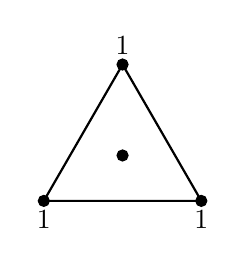
\begin{tikzpicture}
        \draw[fill=black] (-1, 0) circle (2pt) node[below] {$1$};
        \draw[fill=black] (1, 0) circle (2pt) node[below] {$1$};
        \draw[fill=black] (0, 1.732) circle (2pt) node[above] {$1$};
        \draw[thick] (-1, 0) -- (1, 0) -- (0, 1.732) -- cycle;
        \draw[fill=black] (0, .577) circle (2pt);
      \end{tikzpicture}
    \end{subfigure}
    \caption{Illustrating the correspondence between the coloring of a simplex and the degree of its vertex in the auxiliary graph in the case $n = 2$, where the number beside each vertex denotes its color, and we consider the face of $\Delta^2$ colored by $1$ and $2$. Therefore, a simplex is rainbow if and only if its vertex has odd degree.}
    \label{fig:corr}
  \end{figure}
\end{proof}

\subsection{The KKM Theorem}

\begin{theorem}[Knaster, Kuratowski, and Mazurkiewicz, 1929]
  Let $A_1, \ldots, A_{n + 1}$ be closed subsets of $\Delta^n$ such that for any face $\sigma$ of $\Delta^n$, we have $\sigma \subseteq \bigcup_{e_i \in \sigma} A_i$. Then
  $$ \bigcap_{i = 1}^{n + 1} A_i \neq \emptyset. $$
\end{theorem}

Figure \ref{fig:kkm} gives an illustration of the KKM theorem.

\begin{figure}[h]
  \centering
  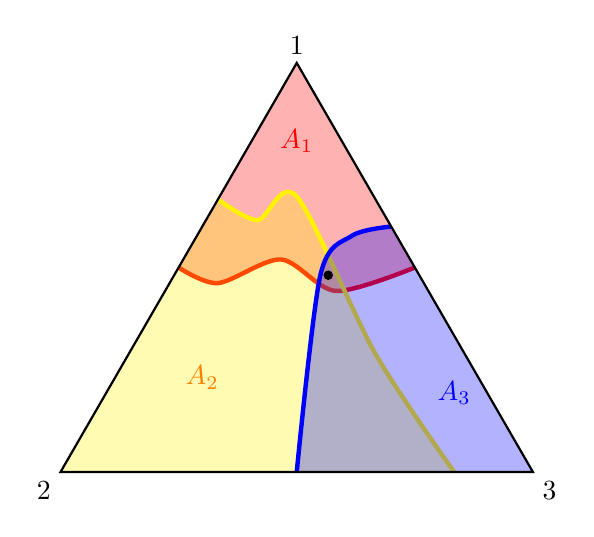
\begin{tikzpicture}
    \node[below left] at (-3, 0) {$2$};
    \node[below right] at (3, 0) {$3$};
    \node[above] at (0, 5.176) {$1$};
    \draw[fill=red, opacity=.3] (0, 5.196) -- plot[smooth] coordinates {(-1.5, 2.598) (-1, 2.4) (-.2, 2.7) (.5, 2.3) (1.5, 2.598)};
    \draw[ultra thick, red] plot[smooth] coordinates {(-1.5, 2.598) (-1, 2.4) (-.2, 2.7) (.5, 2.3) (1.5, 2.598)};
    \draw[fill=yellow, opacity=.3] (-3, 0) -- plot[smooth] coordinates {(-1, 3.4641) (-.5, 3.2) (0, 3.5) (1, 1.5) (2, 0)};
    \draw[ultra thick, yellow] plot[smooth] coordinates {(-1, 3.4641) (-.5, 3.2) (0, 3.5) (1, 1.5) (2, 0)};
    \draw[fill=blue, opacity=.3] (3, 0) -- plot[smooth] coordinates {(0, 0) (.3, 2.5) (.7, 3) (1.2, 3.118)};
    \draw[ultra thick, blue] plot[smooth] coordinates {(0, 0) (.3, 2.5) (.7, 3) (1.2, 3.118)};
    \draw[thick] (-3, 0) -- (3, 0) -- (0, 5.196) -- cycle;
    \node[red] at (0, 4.2) {$A_1$};
    \node[orange] at (-1.2, 1.2) {$A_2$};
    \node[blue] at (2, 1) {$A_3$};
    \draw[fill=black] (.4, 2.5) circle (1.5pt);
  \end{tikzpicture}
  \caption{Illustrating the KKM theorem.}
  \label{fig:kkm}
\end{figure}

We prove the KKM theorem from Brouwer's fixed point theorem.

\begin{proof}
  For each $i \in [n + 1]$, let $g_i : \Delta^n \to \RR$ be defined by $g_i(x) = \dist(x, A_i)$, where $\dist(x, A_i)$ denotes the distance between $x$ and $A_i$. Then $g_i$ is continuous for each $i \in [n + 1]$.

  Let $f : \Delta^n \to \Delta^n$ be defined as follows. Let $x = (x_1, \ldots, x_{n + 1}) \in \Delta^n$. Then $x_i \geq 0$ for each $i \in [n + 1]$ and $\sum_{i = 1}^{n + 1} x_i = 1$. Define
  $$ f(x) = \frac{\left(x_1 + g_1(x), \ldots, x_{n + 1} + g_{n + 1}(x)\right)}{1 + \sum_{i = 1}^{n + 1} g_i(x)}. $$
  Then $f$ is continuous.

  By Brouwer's fixed point theorem, there exists $z = (z_1, \ldots, z_{n + 1}) \in \Delta^n$ such that $f(z) = z$. Let $S(z) = \{ i \in [n + 1] : z_i > 0 \}$, i.e., $S(z)$ is the set of the indices of the vertices of $\supp(z)$. By the condition of the KKM theorem,
  $$ z \in \conv(\supp(z)) \subseteq \bigcup_{i \in S(z)} A_i. $$
  Hence, there exists $i \in S(z)$ such that $z \in A_{i_0}$, so $g_{i_0}(z) = 0$. Since $f(z) = z$, then the $i_0^\text{th}$ coordinate of $f(z)$ equals $z_{i_0}$. Therefore,
  $$ z_{i_0} = \frac{z_{i_0} + g_{i_0}(z)}{1 + \sum_{i = 1}^{n + 1} g_i(z)} = \frac{z_{i_0}}{1 + \sum_{i = 1}^{n + 1} g_i(z)}. $$
  Since $z_{i_0} > 0$, then
  $$ 1 = \frac{1}{1 + \sum_{i = 1}^{n + 1} g_i(z)}. $$
  This implies that $\sum_{i = 1}^{n + 1} g_i(z) = 0$, so $g_i(z) = 0$ for each $i \in [n + 1]$. For each $i \in [n + 1]$, since $A_i$ is closed, then $z \in A_i$. This completes the proof.
\end{proof}

\end{document}
